\section{Funzionalità offerte}
L'applicazione prevede la presenza di un Wallet associato a ciascun tenant, che pu\`o essere ricaricato tramite pagamenti effettuati con \textit{Stripe}.
All'interno del sistema sono previsti dei \textit{workflow}, processi che utilizzano dati provenienti da banche dati esterne per effettuare analisi di vario tipo.
Ogni operazione all'interno del workflow ha un costo, e per ognuna di queste viene scalato un determinato importo in base a un listino prezzi associato al tenant di appartenenza dell'utente.
Quando un'operazione viene inserita nella coda pagamenti, questa viene registrata nel database e il relativo importo viene scalato automaticamente dal Wallet del tenant.

All'interno dell'interfaccia sono predisposte due schermate, una per la gestione del Wallet e

\section{Sezione gestione Wallet}
L'utente ha a disposizione una dashboard per monitorare il Wallet del suo tenant di appartenenza in cui può visualizzare lo storico dei movimenti e caricare il Wallet.

\begin{figure}[H]
  \centering
  \includegraphics[width=8.5cm]{images/gestione-wallet/mock-gestione-wallet.png}
  \caption{Mock realizzato in Figma della schermata di Gestione Wallet}
\end{figure}

Nella parte superiore abbiamo dei widget che riportano in alcuni parametri in modo da essere facilmente visualizzabili:
\begin{enumerate}
  \item Credito disponibile
  \item Credito speso, con andamento in relazione al mese precedente
  \item Credito depositato, con andamento in relazione al mese precedente
  \item Differenza tra credito speso e credito depositato, con andamento in relazione al mese precedente.
\end{enumerate}

Abbiamo un bottone che apre una modale che ti permette di selezionare un importo arbitrario:

\begin{figure}[H]
  \centering
  % \includegraphics[width=8.5cm]{images/mock-gestione-wallet.png}
  \caption{Mock della modale per ricaricare}
\end{figure}

\section{Sezione gestione listini prezzi}

\section{Considerazioni metodi di pagamento}
